\documentclass{beamer}
\mode<presentation>

\setbeamertemplate{navigation symbols}{}
\setbeamertemplate{theorems}[numbered]
\setbeamertemplate{items}[default]
\setbeamercovered{dynamic}
\setlength{\unitlength}{1cm}
\setbeamertemplate{footline}[frame number]
% \setbeamercolor{background canvas}{bg=gray}

\usepackage{setspace}
\usepackage{amsmath,amssymb}
\usepackage{amsthm}
\usepackage{pgf,pgfarrows}
% \usepackage[cp1250]{inputenc}
\usepackage[utf8x]{inputenc}
\usepackage[polish]{babel}
% \usepackage{polski}
% \let\lll\undefined
% \selectlanguage{polish}
\usepackage[T1]{fontenc}
\usepackage{graphics}
\usepackage{tikz,lipsum,lmodern}
% \usepackage{algorithm}
\usepackage[ruled]{algorithm}
% \usepackage[ruled,vlined,linesnumbered,longend,algochapter]{algorithm2e}
\usepackage{algpseudocode}
\usepackage{scalefnt}
\usepackage{array}
\usepackage{colortbl}
\usepackage{tabularx}
\usepackage[most]{tcolorbox}
\usepackage[font=scriptsize,labelfont=bf]{caption}
% \usepackage[demo]{graphicx}
% \usepackage{caption}
% \usepackage{subcaption}

\usetikzlibrary{arrows,automata,snakes}
\usetheme{Frankfurt}
\usecolortheme{seahorse} %crane
\useinnertheme{circles}


\newtheorem*{lemat}{Lemat}
\newtheorem{twierdzenie}{Twierdzenie}
\newtheorem{definicja}{Definicja}
\newcommand{\myitem}{\item[$\vartriangleright$]}
\newcommand{\nota}[1]{{\color{gray} \emph{#1}}}
\newcommand{\HarmonicN}[1]{H_{#1}}
\newcommand{\BALL}[2]{\mathbf{B}(#1,#2)}
\newcommand{\DISC}[2]{\mathbf{D}(#1,#2)}
\newcommand{\SPHERE}[2]{\mathbf{S}(#1,#2)}
\newcommand{\BigO}[1]{\mathcal{O}\left(#1\right)}
\newcommand{\BigTh}[1]{\Theta\left(#1\right)}
\newcommand{\slfrac}[2]{\left.#1\middle/#2\right.}
\newcommand{\PR}[1]{\mathrm{Pr}\left[#1\right]}
\newcommand{\E}[1]{\mathbb{E}\left[#1\right]}
\newcommand{\var}[1]{\mathbb{V}\mathrm{ar}\left[#1\right]}
\newcolumntype{C}{>{\centering\arraybackslash}p{0.5cm}}
\newcolumntype{Y}{>{\columncolor{blue!5}}C}

%\pgfpagesuselayout{4 on 1 with notes}[a4paper,border shrink=3mm]


\title{Algorytm Minimax dla gry w Warcaby}

\author{
	\textbf{Janusz Witkowski}
	\newline \newline
	Praca napisana pod kierunkiem \textbf{dra Macieja Gębali}
}

\date{Grudzień 2022, Wrocław}


\begin{document}

\begin{frame}[plain]{}
	\titlepage
\end{frame}


\section{Warcaby}
\begin{frame}{Warcaby}

	Warcaby są XII-wieczną grą dwuosobową o doskonałej informacji i sumie zerowej.
	W Warcabach gracze na zmianę poruszają się dwoma różnymi typami figur (pionami i damkami) po ukosach, a celem gry jest uniemożliwienie ruchu przeciwnikowi.

	\begin{figure}
		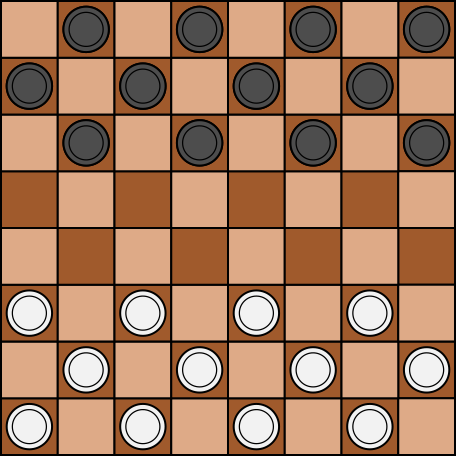
\includegraphics[scale=.4]{figures/warcaby_planszaStartowa.png}
		\caption{Plansza startowa w Warcabach}
	\end{figure}

\end{frame}
	% warcaby
\begin{frame}{Wariant angielski}

	% \hspace{1cm}

	% \begin{definicja}[Ezoteryczny język programowania]
	% 	Język zaprojektowany do badania niekonwencjonalnych technik programowania.
	% 	Taki język nie jest przeznaczony do pisania praktycznych aplikacji, mimo to jest \textbf{zupełny w sensie Turinga} (da się w nim zasymulować każdy możliwy program).
	% \end{definicja}

	Praca rozpatruje szczególną wersję Warcabów - \textbf{wariant angielski}.
	Wariant ten wprowadza dwie zmiany:
	\begin{itemize}
		\myitem Piony nie mogą poruszać się do tyłu,
		\myitem Damki nie ruszają się na dystansy większe niż jedno pole.
	\end{itemize}

	\begin{columns}
		\begin{column}{.5\hsize}
			{\centering
			\begin{figure}
				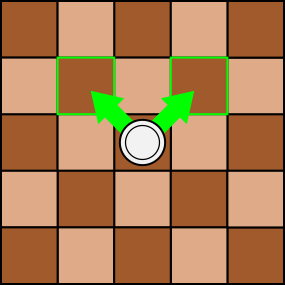
\includegraphics[scale=.25]{figures/warcaby_ruchyPionZwykle3.png}
				\caption{Ruchy dla piona}
			\end{figure}
			}
		\end{column}
		\begin{column}{.5\hsize}
			{\centering
			\begin{figure}
				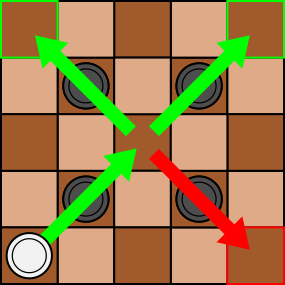
\includegraphics[scale=.25]{figures/warcaby_ruchyPionBicia.png}
				\caption{Bicia dla piona}
			\end{figure}
			}
		\end{column}
	\end{columns}

	\begin{columns}
		\begin{column}{.5\hsize}
			{\centering
			\begin{figure}
				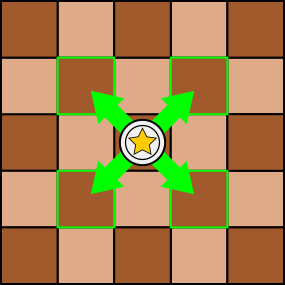
\includegraphics[scale=.25]{figures/warcaby_ruchyDamkaZwykle.png}
				\caption{Ruchy dla damki}
			\end{figure}
			}
		\end{column}
		\begin{column}{.5\hsize}
			{\centering
			\begin{figure}
				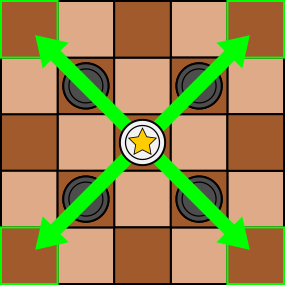
\includegraphics[scale=.25]{figures/warcaby_ruchyDamkaBicia.png}
				\caption{Bicia dla damki}
			\end{figure}
			}
		\end{column}
	\end{columns}

	% \begin{figure}
	% 	\centering
	% 	\begin{subfigure}{.5\textwidth}
	% 	  \centering
	% 	  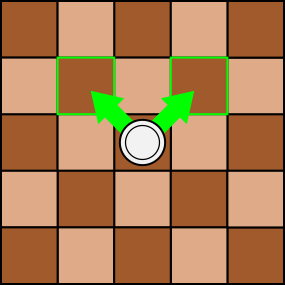
\includegraphics[scale=.6]{figures/warcaby_ruchyPionZwykle3.png}
	% 	  \caption{Legalne ruchy}
	% 	\end{subfigure}%
	% 	\begin{subfigure}{.5\textwidth}
	% 	  \centering
	% 	  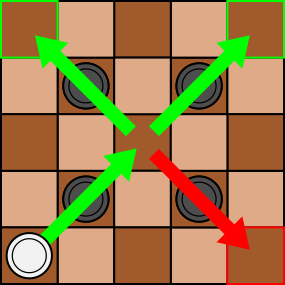
\includegraphics[scale=.6]{figures/warcaby_ruchyPionBicia.png}
	% 	  \caption{Legalne bicia}
	% 	\end{subfigure}
	% 	\caption{Zestaw możliwych ruchów dla piona w wariancie angielskim}
	% \end{figure}
		
	% \begin{figure}
	% 	\centering
	% 	\begin{subfigure}{.5\textwidth}
	% 	  \centering
	% 	  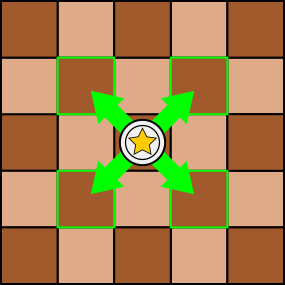
\includegraphics[scale=.6]{figures/warcaby_ruchyDamkaZwykle.png}
	% 	  \caption{Legalne ruchy}
	% 	\end{subfigure}%
	% 	\begin{subfigure}{.5\textwidth}
	% 	  \centering
	% 	  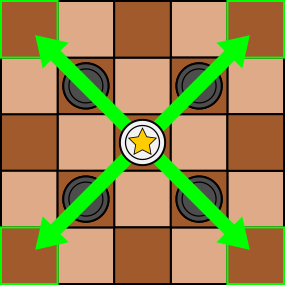
\includegraphics[scale=.6]{figures/warcaby_ruchyDamkaBicia.png}
	% 	  \caption{Legalne bicia}
	% 	\end{subfigure}
	% 	\caption{Zestaw możliwych ruchów dla damki w wariancie angielskim}
	% \end{figure}

	% \vspace{0.6cm}
	% {\hspace{7cm}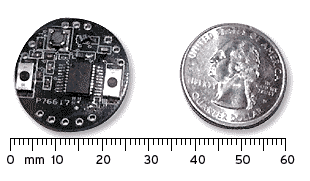
\includegraphics[height=2cm]{figures/mica2.png}}

\end{frame}
	% warcaby

\section{Algorytmy}
% % \begin{frame}[squeeze]{Analiza}
\begin{frame}{Minimax}

  {\large
  \textbf{Minimax} jest algorytmem przeszukiwania przestrzeni stanów rozgrywki dla gier dwuosobowych.
  }

  % {\small
  \begin{itemize}
    \myitem Polega na rekurencyjnym rozpatrywaniu drzew stanów na planszy z perspektyw obu graczy, oznaczonych jako gracz \textit{MAX} oraz gracz \textit{MIN}.
    \myitem Dla stanów na maksymalnej głębokości \textit{h} oblicza się ocenę heurystyczną.
    \myitem \textit{MAX} wybiera ruchy o jak największej wartości oceny, \textit{MIN} - jak najmniejszej.
  \end{itemize}
  % }
  
    

  % \begin{itemize}
  %   \myitem Wouter van Oortmerssen, 1993
  %   \myitem Powstał w dwóch celach:
  %   \begin{itemize}
  %     \item Jak najmniejszy kompilator (1024B);
  %     \item Jak najbardziej zaciemniona składnia.
  %   \end{itemize}
  %   \myitem Używa zmiennych, arytmetyki stosowej, wyrażeń lambda itd.
  % \end{itemize}

  % \begin{figure}
  %   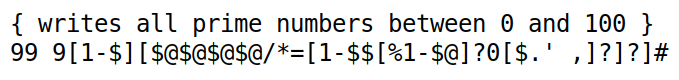
\includegraphics[width=10cm]{figures/false.png}
  % \end{figure}

	% \begin{itemize}
	% \item[$d(u,v)$] --  długość ścieżki z $u$ do $v$
	% \item[$\SPHERE{v}{r}$] $= \{u: d(u,v) = r\}$
	% \item[$\DISC{v}{r}$] $ = \{u: d(u,v)\leq r\}$
	% \end{itemize}

	%  \begin{tikzpicture}[remember picture, overlay]
 	
         \node [shift={(9cm,-3.4cm)}]  at (current page.north west)
            {
            \tikzstyle{place}=[circle,draw=black!100,fill=blue,thin, inner sep=0pt,minimum size=2mm]
            \tikzstyle{red place}=[circle,draw=black!100,fill=yellow!100,thin, inner sep=0pt,minimum size=2mm]

            \begin{tikzpicture}


                \node at (-1,0) [red place]  (1) {};
                \node at (-0.6,0.8) [red place]  (2) {};
                \node at ( -0.1,0.6) [red place]  (3) {};
                \node at ( -0.4,-0.5) [red place]  (4) {};
                \node at ( 0,0) [ red place]  (5) {v};
                \node at (0.75,-0.75) [red place]  (6) {};
                \node at ( 1,0.3) [red place] (7) {};
                \node at (1.5,-0.35) [red place]  (8) {};
                \node at (0.1,-0.85) [red place]  (9) {};


                \node at ( -1.5,-0.3) [place]  (10) {};
                \node at ( -1.5,0.5) [place]  (11) {};
                \node at ( -1.2,1) [place]  (12) {};
                \node at ( -0.2,1.2) [place]  (13) {};
                \node at ( 0.8,0.8) [place]  (14) {};
                \node at ( 1.6,0.6) [place]  (15) {};
                \node at ( 1.9,-0.8) [place]  (16) {};
                \node at ( 1.9,0) [place]  (17) {};
                \node at ( -0.3,-1.2) [place]  (18) {};
                \node at ( 0.5,-1.3) [place]  (19) {};


                \draw [->] (1) to (2);
                \draw [->] (2) to (3);
                \draw [<-] (3) to (7);
                \draw [->] (3) to (5);
                \draw [<-] (5) to (6);
                \draw [<-] (6) to (8);
                \draw [->] (8) to (7);
                \draw [<-] (5) to (4);
                \draw [->] (1) to (4);
                \draw [<-] (6) to (9);
                \draw [<-] (4) to (9);

                \draw [<-] (1) to (10);
                \draw [<-] (1) to (11);
                \draw [<-] (2) to (12);
                \draw [<-] (2) to (13);
                \draw [<-] (7) to (14);
                \draw [<-] (7) to (15);
                \draw [<-] (8) to (16);
                \draw [<-] (8) to (17);
                \draw [<-] (9) to (18);
                \draw [<-] (9) to (19);


          
            \end{tikzpicture}

            };
        
\end{tikzpicture}

	% \vspace{2cm}	

  %   \begin{twierdzenie}[Propagacja minimum]
  %   	Niech $M_{v,r}$  oznacza zdarzenie, że $v$ nadaje w rundzie $r$ oraz
  %       niech $\mathcal{G} =(V,E)$ będzie graf skierowanym i niech $v\in V$.
  %       Załóżmy, że $\SPHERE{v}{r}\neq \emptyset$.
  %       Wówczas zdarzenia $M_{v,0}, \ldots M_{v,r}$ \underline{są niezależne}
  %       oraz
  %       $$
  %         \Pr[M_{v,j}] = |\SPHERE{v}{j}|\Big/{|\DISC{v}{j}|}~.
  %       $$
  %   \end{twierdzenie}

\end{frame}
	% minimax
% \begin{frame}[squeeze]{}
\begin{frame}{Minimax (przykład)}
	
	{\centering
	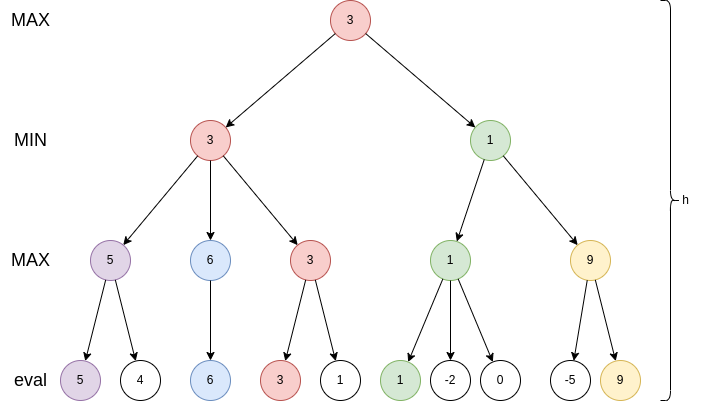
\includegraphics[width=11cm]{figures/minimax3.png}
	}

\end{frame}

	% minimax przyklad
\begin{frame}{Funkcja oceny heurystycznej}

	\[ F(S) = \sum_{i=1}^{n} param_i(S) * weight_i \]

	\begin{table}[h]
		\centering
		{\small
		\begin{tabular}{|c|c|c|}
		\hline
			\textit{i} & \textit{param} & \textit{weight} \\ 
		\hline
			1 & Liczba sojuszniczych pionów & 15\\ 
		\hline
			2 & Liczba przeciwnych damek przy ścianie & -123\\ 
		\hline
			3 & Liczba możliwych ruchów gracza & 0 \\
		\hline
			4 & Czy pion przeciwnika znajduje się w kącie & 47 \\
		\hline
			\ldots & \ldots & \ldots \\
		\hline
		\end{tabular}
		}
		\caption{Przykładowe parametry z przykładowymi wagami.}
	\end{table}

\end{frame}


	% ocena
\begin{frame}{Algorytm genetyczny}

	\begin{itemize}
		\myitem Celem pracy jest wyznaczenie jak najlepszego ciągu wag do funkcji oceny heurystycznej.
		% \myitem Ludzka intuicja może w tym zadaniu zawieść.
		\myitem Pomysł: zastosowanie algorytmu genetycznego.
	\end{itemize}
	
	\hspace{1cm}

	\textbf{Algorytm genetyczny} symuluje dobór naturalny w przyrodzie. Na~populacji osobników (zbiorze rozwiązań problemu) wykonuje~się operacje:
	\begin{enumerate}
		\item Ewaluacja osobników
		\item Selekcja zbioru rodziców
		\item Krzyżowanie 
		\item Losowe mutacje
		\item Tworzenie nowej populacji
	\end{enumerate}
	
	% \begin{columns}	
			
	% 	\begin{column}{.45\hsize}
			
	% 		\begin{tikzpicture}[remember picture, overlay]
	% 			\node [shift={(2.2 cm,-4.5cm)}]  at (current page.north west)
	% 			{
	% 				\tikzstyle{place}=[circle,draw=blue!50,fill=blue!20,thick,inner sep=0pt,minimum size=4mm]
	% 				\tikzstyle{red place}=[circle,draw=red!50,fill=yellow,thick,inner sep=0pt,minimum size=4mm]
					
	% 				{\scalefont{0.6}
						
	% 					\begin{tikzpicture}
							
	% 						\only<1>{
	% 							\node at (-1,1) [place]  (1) {$0.45$};
	% 							\node at (-1,3) [place]  (2) {$0.76$};
	% 							\node at ( 0,2) [place]  (3) {$0.49$};
	% 							\node at ( 0.2,0) [place]  (4) {$0.78$};
	% 							\node at (1.5,2.5) [place]  (6) {$0.67$};
	% 							\node at ( 2,-0.2) [place] (7) {$0.86$};
	% 							\node at (2.5,1.7) [place]  (8) {$0.22$};}
							
	% 						\only<1,2>{
	% 							\node at ( 1,1) [ red place] (5) {$0.01$};}
							
	% 						\only<2>{
	% 							\node at (-1,1) [red place] (1) {$0.01$};
	% 							\node at (-1,3) [red place]  (2) {$0.01$};
	% 							\node at ( 0,2) [red place](3) {$0.01$};
	% 							\node at ( 0.2,0) [red place]  (4) {$0.01$};
	% 							\node at (1.5,2.5) [red place] (6) {$0.01$};
	% 							\node at ( 2,-0.2) [red place](7) {$0.01$};
	% 							\node at (2.5,1.7) [red place]  (8) {$0.01$};}
							
	% 						\draw [->,-latex] (1) to (2);
	% 						\draw [<->,-latex] (2) to (3);
	% 						\draw [<->,-latex]  (3) to (6);
	% 						\draw [<->,-latex]  (3) to (5);
	% 						\draw [<->,-latex]  (5) to (6);
	% 						\draw [->,-latex]  (6) to (8);
	% 						\draw [->,-latex]  (8) to (7);
	% 						\draw [->,-latex]  (7) to (5);
	% 						\draw [->,-latex]  (5) to (4);
	% 						\draw [<->,-latex]  (1) to (4);
							
	% 					\end{tikzpicture}
	% 				}
	% 			};
	% 		\end{tikzpicture}
			
	% 	\end{column}		
		
	% 	\begin{column}{.75\hsize}		
				
	% 			\textbf{Model}
	% 			\begin{enumerate}
	% 				\myitem model sieci: graf skierowany $\mathcal{G}=(V,E)$
	% 				\myitem każda stacja $v_i \in V$ losuje $x_i\in[0,1]$
	% 			\end{enumerate}
				
	% 			\vspace{0.4cm}
				
	% 			\textbf{Cel}
	% 			\begin{enumerate}
	% 				\myitem propagacja statystyk pozycyjnych, 
	% 				\newline np. $\min(x_1,\ldots, x_n)$
	% 			\end{enumerate}
				
				
	% 			\vspace{0.4cm}
				
	% 			\textbf{Dlaczego statystyki pozycyjne?}
	% 			\begin{enumerate}
	% 				\myitem zastosowanie do rozproszonego obliczania dowolnej funkcji \textit{separowalnej}\\
	% 			\end{enumerate}
						
	% 	\end{column}
			
	% \end{columns}
	
\end{frame}
	% algorytm genetyczny
% \begin{frame}{Implementacja algorytmu genetycznego}
    \begin{enumerate}
        \item \textbf{Osobniki} \\
        Ciągi wag w postaci tablic liczb całkowitych.
        \item \textbf{Ewaluacja} \\
        Pojedynek każdy-z-każdym (białe/czarne i na odwrót)
        \item \textbf{Selekcja} \\
        Ruletka (lepiej grające osobniki mają większą szansę na przejście)
        \item \textbf{Krzyżowanie} \\
        Pary rodziców mają po dwójce dzieci 
        \item \textbf{Mutacje} \\
        Szansa na wylosowanie nowej wartości losowej wag w ciągu.
    \end{enumerate}
\end{frame}
	% szczegóły genetyka

\section{Implementacja}
\begin{frame}{Język i struktura}

    Projekt został napisany w języku \textbf{JAVA} w wersji \textit{OpenJDK 17.0.4 2022-07-19} (aczkolwiek wykorzystuje funkcjonalności z \textit{OpenJDK 14}).
    
    % \begin{columns}

    %     \begin{column}{.5\hsize}
    %         \begin{itemize}
    %             \myitem Karl Hasselström \& Jon Åslund, 2001
    %             \myitem Program w SPL wygląda jak szekspirowska sztuka
    %             \myitem Postacie to zmienne
    %             \myitem Wielkość zmiennej zależy wykładniczo od liczby przypisanych do niej komplementów lub przywar
    %         \end{itemize}
    %     \end{column}

    %     \begin{column}{.5\hsize}
    %         \begin{figure}
    %             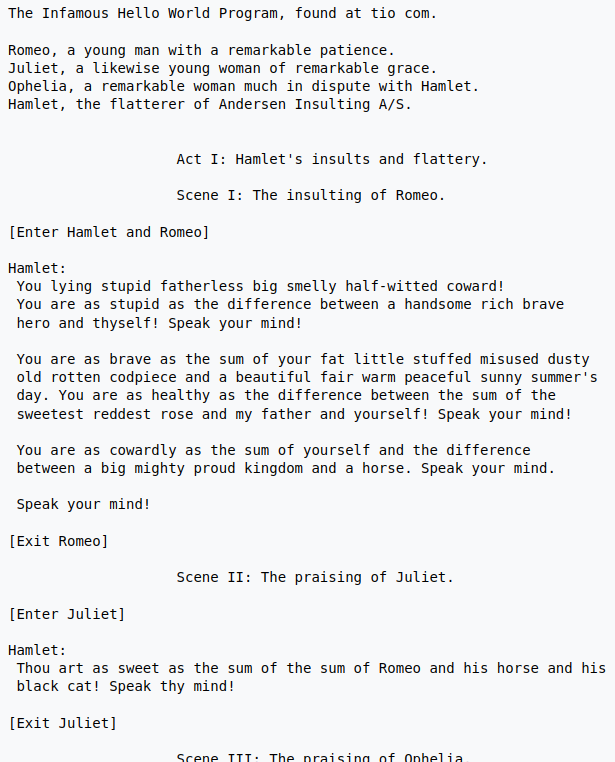
\includegraphics[height=6.3cm]{figures/spl.png}
    %             \caption*{\footnotesize Fragment sztuki ,,Hello World'' {\color{blue} \hyperlink{frame:przypisy}{(5)}}}
    %         \end{figure}
    %     \end{column}

    % \end{columns}

\end{frame}

\begin{frame}{Programy wywoławcze}

	Poniższe programy wywołuje się z linii poleceń z odpowiednimi argumentami.

	\begin{itemize}
		\myitem {\large \textbf{Play}}
		\begin{itemize}
			\item Rozpoczyna rozgrywkę między graczami (każdy z nich może być człowiekiem lub komputerem)
			\item Dla graczy komputerowych należy podać również pliki z ciągiem wag
			\item I/O na poziomie konsoli
		\end{itemize}
		\myitem {\large \textbf{Find}}
		\begin{itemize}
			\item Rozpoczyna sesję algorytmu genetycznego
			\item Może wznowić przedwcześnie przerwaną sesję z pliku populacji
			\item Wynik zapisuje w \textbf{heuristics/output/}
		\end{itemize}
		\myitem {\large \textbf{Show}}
		\begin{itemize}
			\item Nazwa pliku osobnika do wyświetlenia
		\end{itemize}
	\end{itemize}

    % \begin{columns}

	% 	\begin{column}{.4\hsize}
	% 		\begin{figure}
	% 			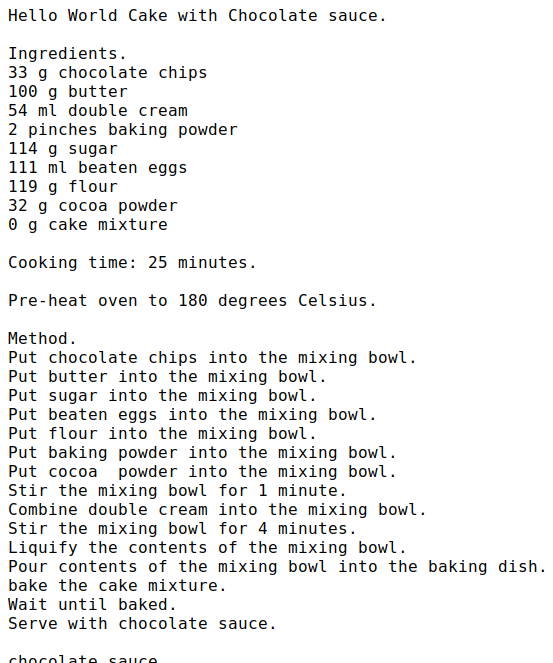
\includegraphics[height=6cm]{figures/chef1.png}
	% 			\caption*{\footnotesize Przepis na ciasto HelloWorld {\color{blue} \hyperlink{frame:przypisy}{(6)}}}
	% 		\end{figure}
	% 	\end{column}

	% 	\begin{column}{.6\hsize}
    %         \hspace{0.5cm}
	% 		\begin{itemize}
	% 			\myitem David Morgan-Mar, 2003
	% 			\myitem Kod źródłowy przypomina przepis kulinarny
	% 			\myitem Niepisanym wyzwaniem jest pisanie programów z których da się też przygotować posiłek
	% 		\end{itemize}
    %         % \begin{figure}
    %         %     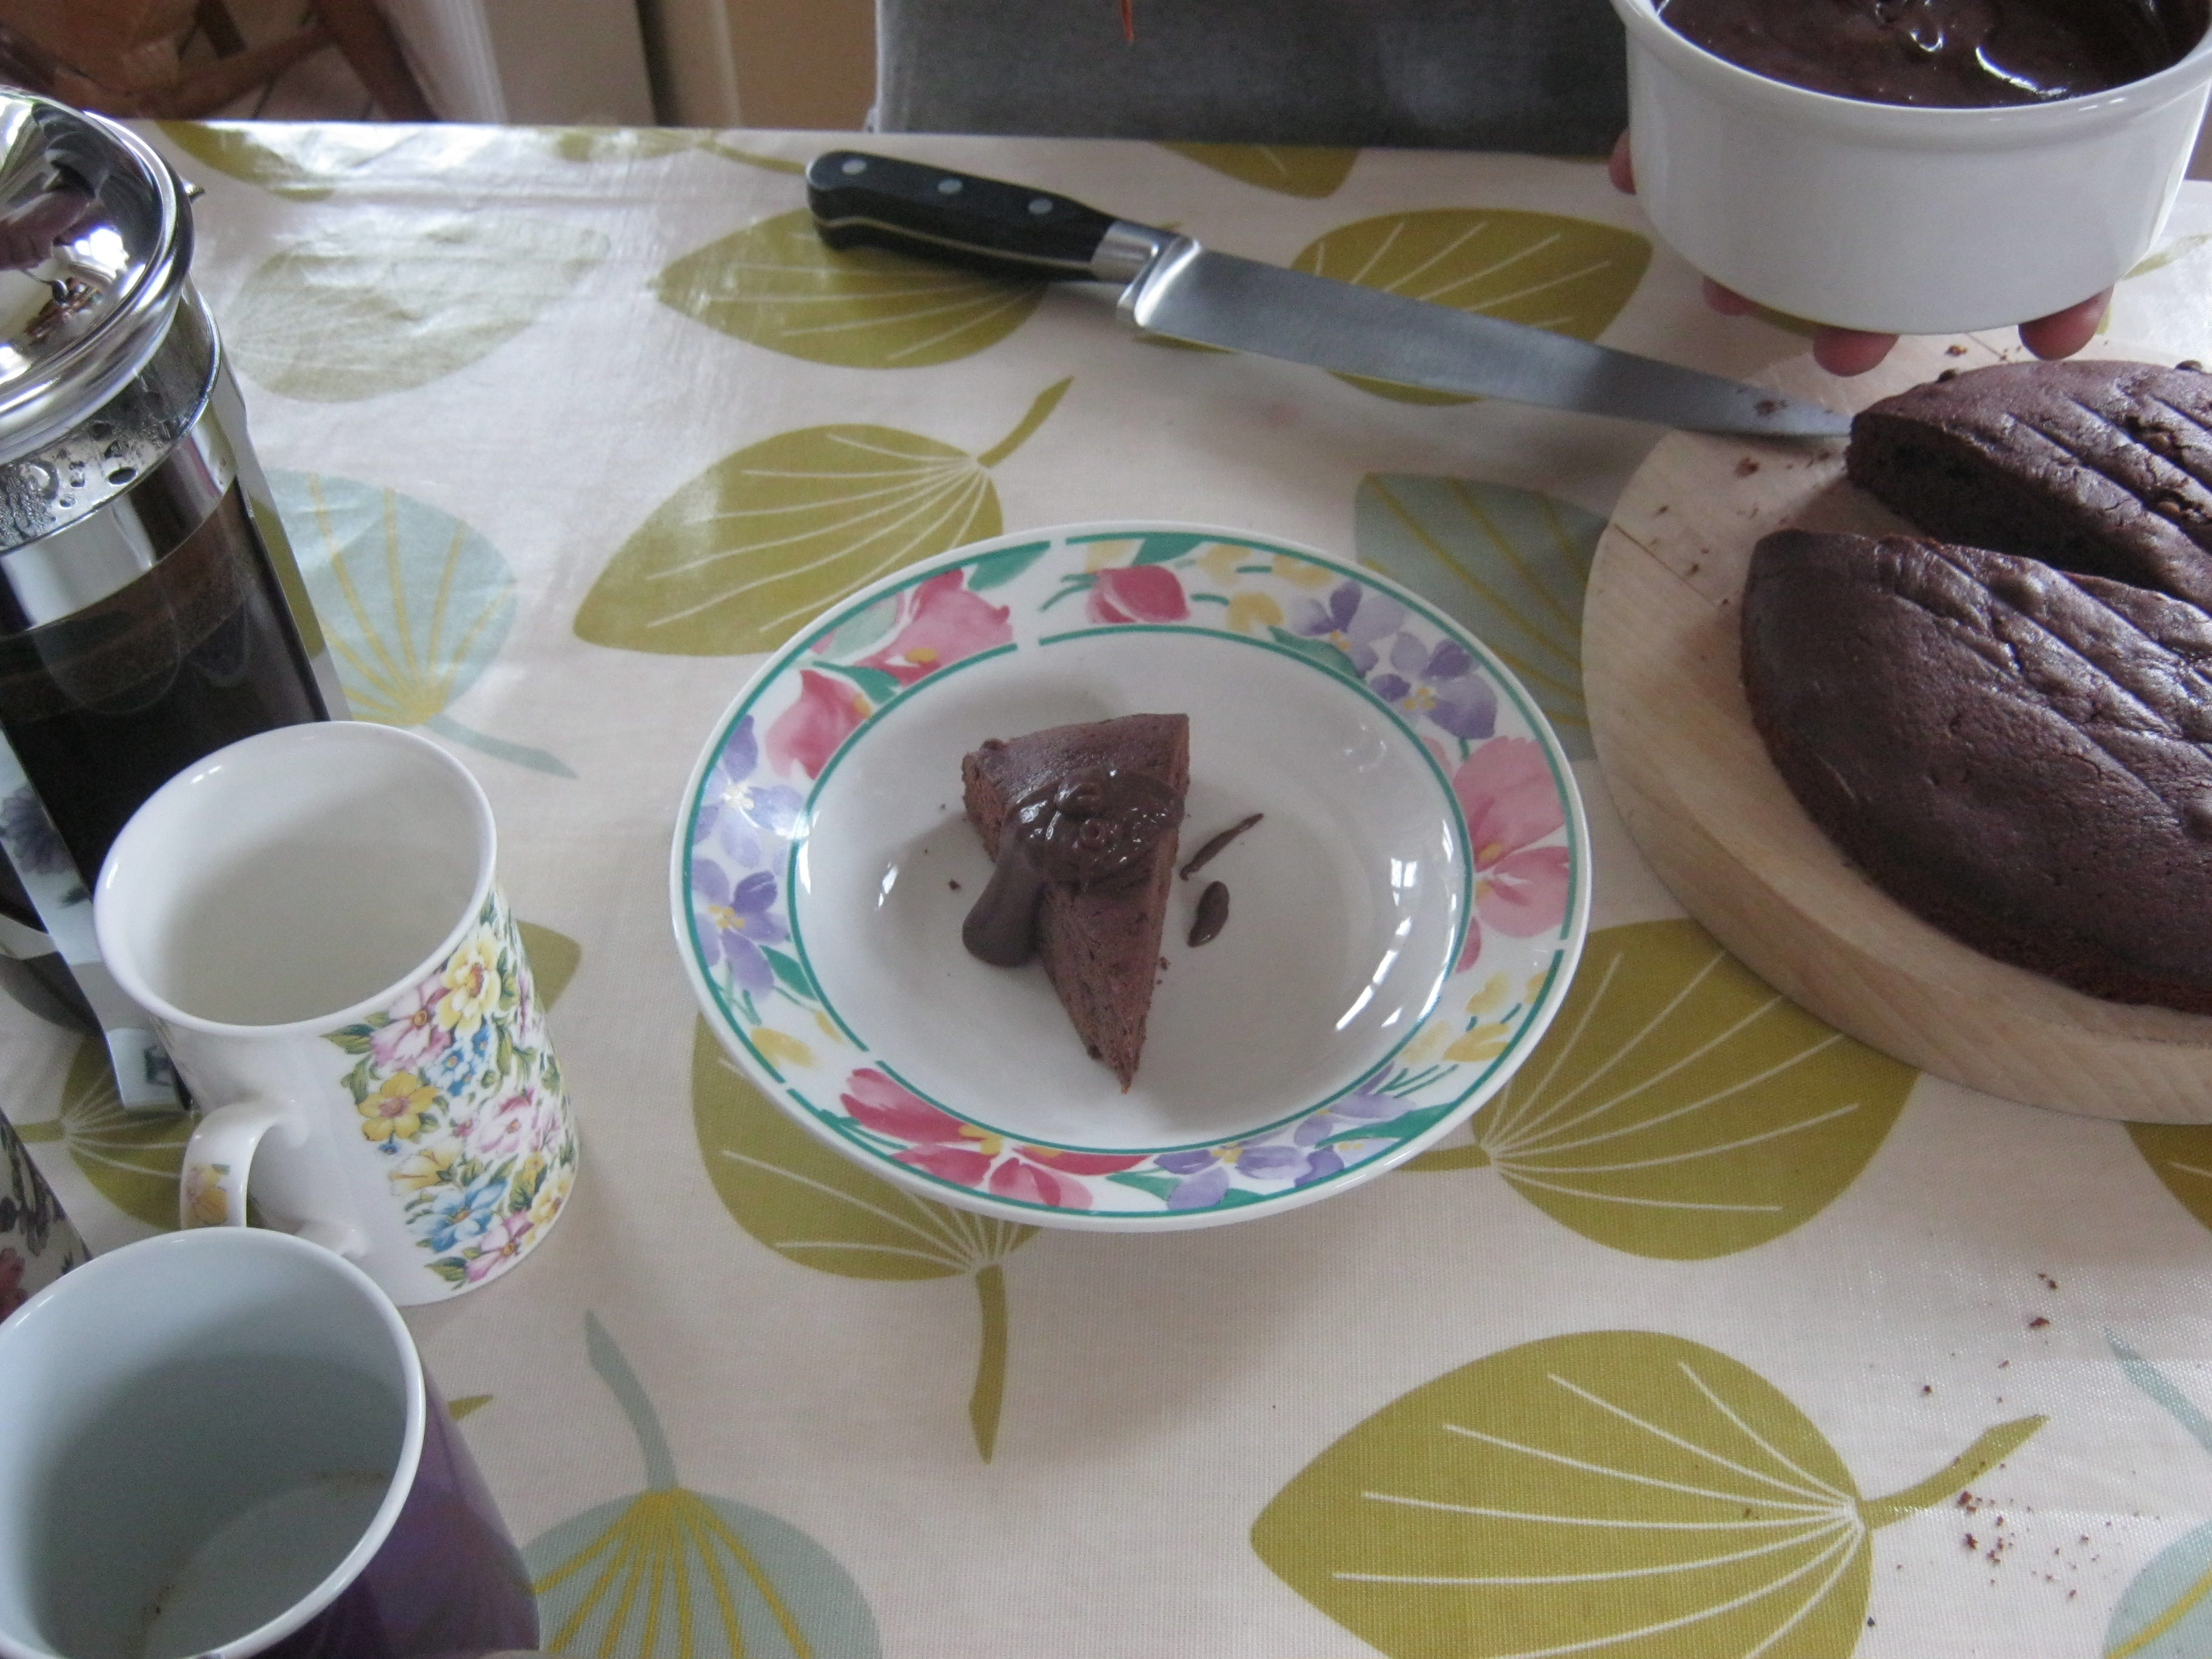
\includegraphics[width=4.5cm]{figures/chef_cake.jpg}
    %         %     \caption{\scriptsize Ciasto ,,HelloWorld'' autorstwa Mike Worth}
    %         % \end{figure}
	% 	\end{column}

	% \end{columns}

\end{frame}

% \begin{frame}{Rockstar}
    \begin{columns}

		\begin{column}{.5\hsize}
            % 
\includegraphics[width=5cm]{figures/rockstar_dev.jpg}
			\begin{itemize}
				\myitem Dylan Beattie, 2018
				\myitem Służy do pisania programów przypominających rockowe piosenki z lat '80
				\myitem Autor języka zagrał piosenkę ze słowami ,,FizzBuzz'' na konferencji Build Stuff 2019
			\end{itemize}
		\end{column}

        \begin{column}{.5\hsize}
			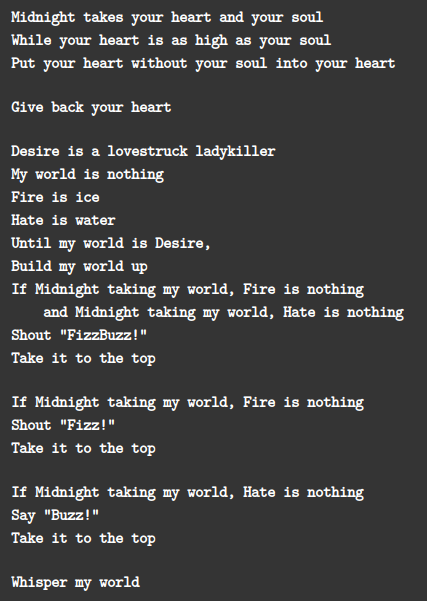
\includegraphics[height=7cm]{figures/rockstar.png}
		\end{column}

	\end{columns}
\end{frame}

% \begin{frame}{Piet}
    % \begin{columns}

	% 	\begin{column}{.5\hsize}
			\begin{itemize}
				\myitem David Morgan-Mar, 2003
				\myitem Zainspirowany abstrakcyjną twórczością Piet'a Mondrian'a
				\myitem Kodem źródłowym jest dwuwymiarowa bitmapa
                \myitem W zależności od różnicy kolorów, ruchomy wskaźnik uruchamia różne komendy i korzysta ze stosu
			\end{itemize}
		% \end{column}

        % \begin{column}{.5\hsize}
			% 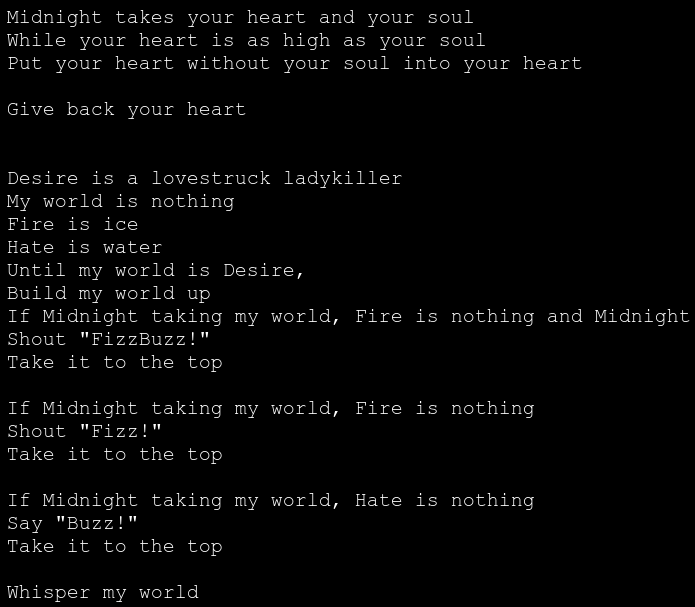
\includegraphics[height=7cm]{figures/rockstar1.png}
		% \end{column}

	% \end{columns}
    \begin{columns}
        \begin{column}{.5\hsize}
            \begin{figure}
                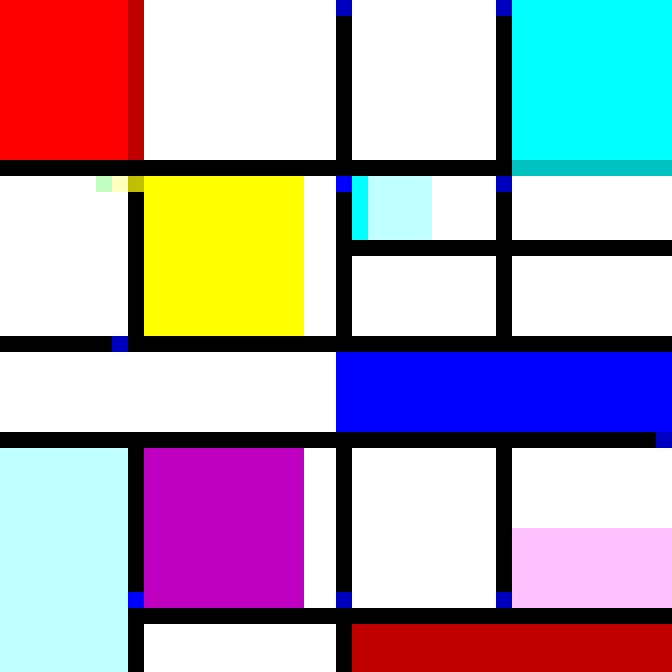
\includegraphics[height=2cm]{figures/piet_piet.png}
                \caption*{\scriptsize Program drukujący ,,Piet''{\color{blue} \hyperlink{frame:przypisy}{(7)}}}
            \end{figure}
        \end{column}
        \begin{column}{.5\hsize}
            \begin{figure}
                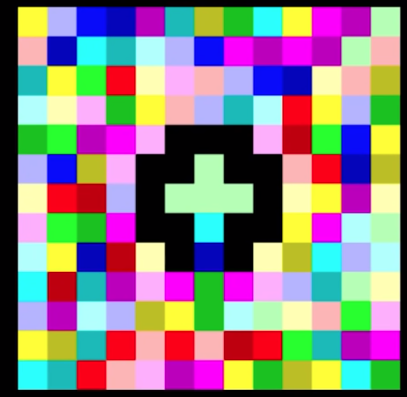
\includegraphics[height=2cm]{figures/piet_helloworld.png}
                \caption*{\scriptsize Program drukujący ,,Hello World!''{\color{blue} \hyperlink{frame:przypisy}{(7)}}}
            \end{figure}
        \end{column}
    \end{columns}


\end{frame}

% \begin{frame}{Inne humorystyczne języki}
    \begin{columns}
        \begin{column}{.6\hsize}
            {\large Folders}
            \begin{itemize}
                \myitem Daniel Temkin, 2015
                \myitem Kodem źródłowym jest struktura folderów
            \end{itemize}
        \end{column}
        \begin{column}{.45\hsize}
            \begin{figure}
                {\hspace{0cm}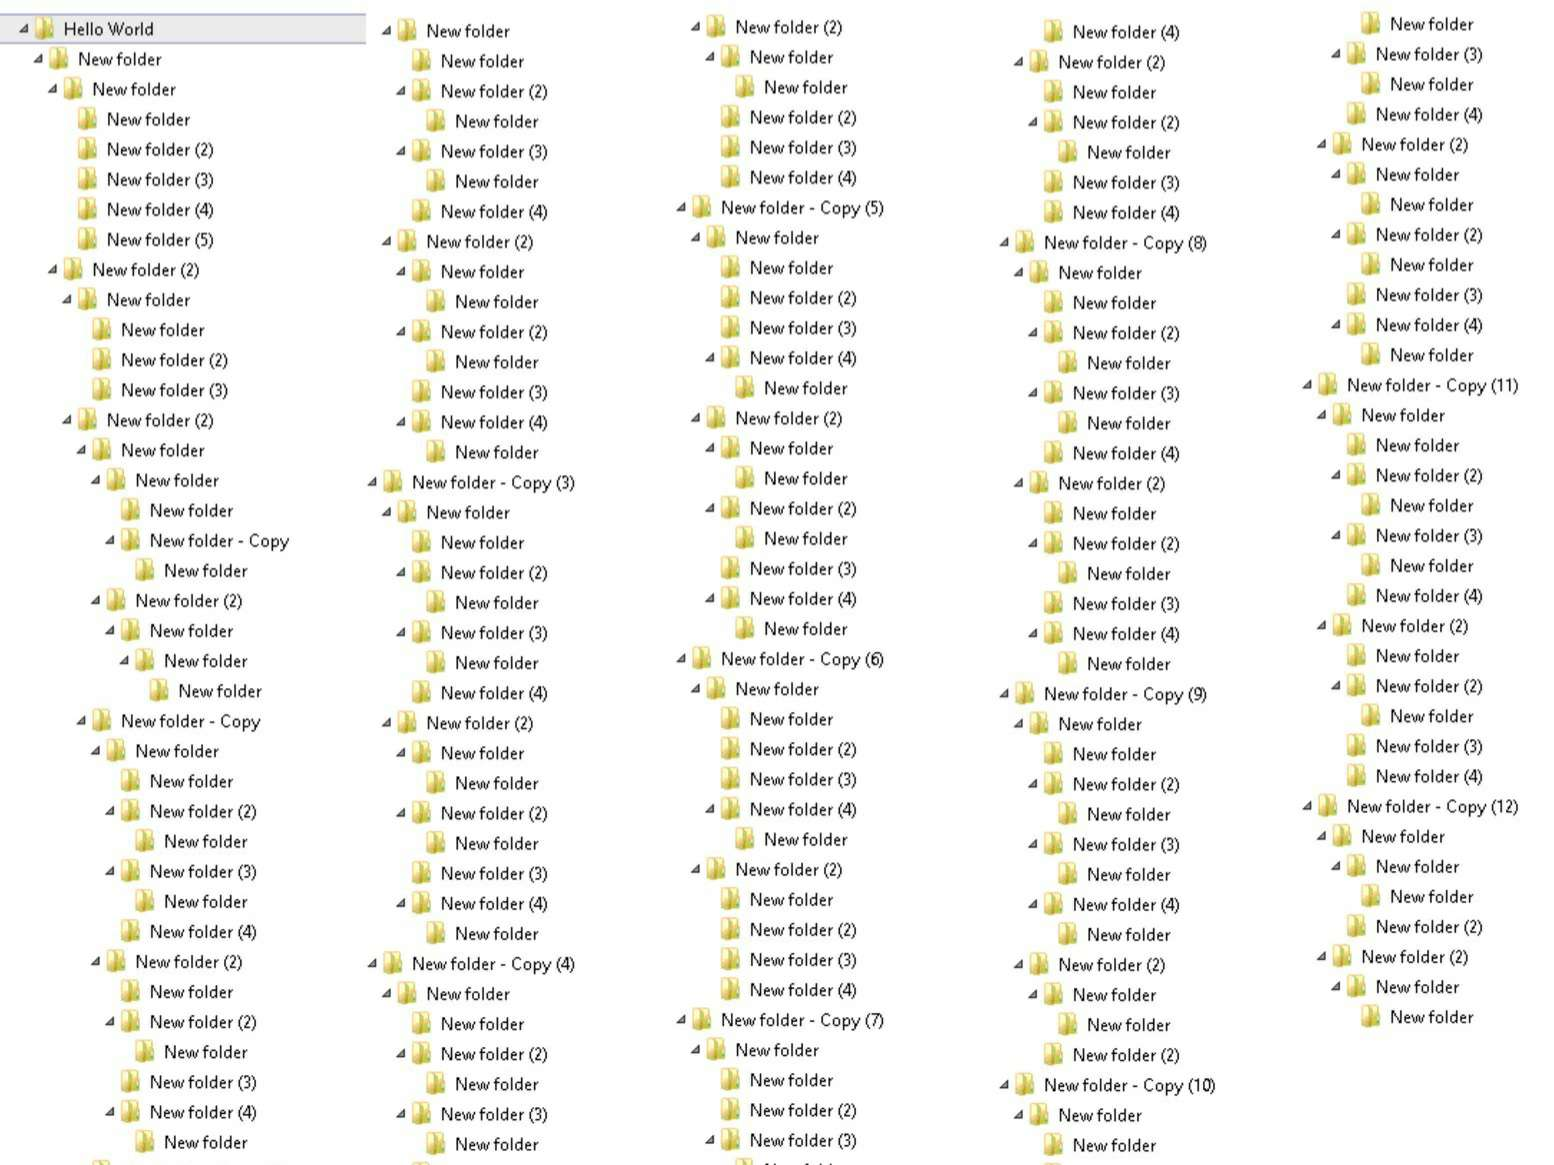
\includegraphics[height=2.5cm]{figures/folders.jpg}}
                \caption*{\scriptsize Folders, ,,Hello World!''{\color{blue} \hyperlink{frame:przypisy}{(8)}}}
            \end{figure}
        \end{column}
    \end{columns}

    \begin{columns}
        \begin{column}{.6\hsize}
            {\large Whitespace}
            \begin{itemize}
                \myitem Edwin Brady \& Chris Morris, 2003
                \myitem Jedynymi rozpoznawanymi znakami są spacja, tab i nowa linia
            \end{itemize}
        \end{column}
        \begin{column}{.45\hsize}
            \begin{figure}
                {\hspace{0cm}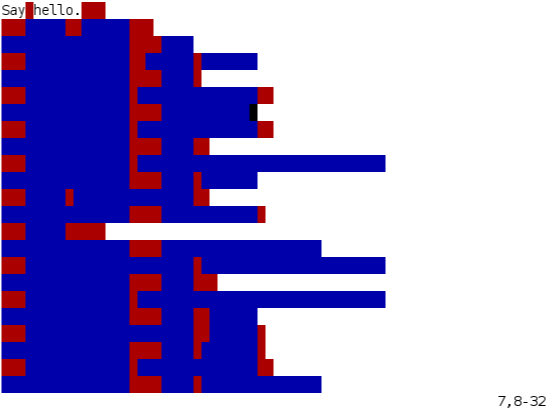
\includegraphics[height=2.5cm]{figures/whitespace.png}}
                \caption*{\scriptsize Whitespace, ,,Hello''{\color{blue} \hyperlink{frame:przypisy}{(9)}}}
            \end{figure}
        \end{column}
    \end{columns}

    % \begin{columns}
    %     \begin{column}{.65\hsize}
    %     \end{column}
    % \end{columns}
\end{frame}

\section{Wyniki}
\begin{frame}{Wyniki: wagi parametrów}

    \textbf{Cel eksperymentu:} Poznać względne wagi wszystkich parametrów; sprawdzić które parametry nie mają znaczenia w rozgrywce (waga bliska zeru).

    \textbf{Wyniki:}
    \begin{itemize}
        % \myitem Najważniejszymi parametrami w rozgrywce okazały się \textit{X, Y, Z (omówienie)}.
        % \myitem Najgorzej punktowane parametry to \textit{A, B, C (omówienie)}.
        % \myitem Najmniejszy wpływ na grę mają parametry \textit{U, V, W (omówienie)}. Będzie można odpuścić te parametry w następnych eksperymentach.
        \myitem Mocno ujemna waga dla sojuszniczych pionów (przewrażliwienie).
        \myitem Zwrócenie uwagi na mobilność figur na planszy.
        \myitem Powstała strategia jest agresywna i dąży do jak najszybszego awansu do damek.
    \end{itemize}

\end{frame}

\begin{frame}{Wyniki: różne głębokości}

    \textbf{Cel eksperymentu:} Sprawdzić czy puszczenie dwóch sesji algorytmu genetycznego z różnymi głębokościami przeszukiwań (odpowiednio 4 i 5) dają różne rezultaty.

    \textbf{Wyniki:}
    \textit{TBA}.
    % \begin{itemize}
    %     \myitem
    % \end{itemize}

    % \textbf{Zadanie:} Napisz program który stwierdzi czy dana liczba naturalna jest pierwsza.

    % \vspace*{0.5cm}

    % \begin{tcolorbox}[title={C, 61 Bajtów {\color{blue} \hyperlink{frame:przypisy}{(10)}}}]
    %     % r;main(i,j){r=(--i>1);for(j=i-1;j>1;)r*=!!(i\%j--);return r;}
    %     {
\includegraphics[width=11cm]{figures/primes_c.png}}
    % \end{tcolorbox}

    % \begin{tcolorbox}[title={Perl, 25 Bajtów {\color{blue} \hyperlink{frame:przypisy}{(11)}}}]
    %     % \$\_=2==grep\$'\%\$\_<1,//..\$\_
    %     {
\includegraphics[width=11cm]{figures/primes_perl.png}}
    % \end{tcolorbox}

    % \begin{tcolorbox}[title={APL, 13 Bajtów {\color{blue} \hyperlink{frame:przypisy}{(12)}}}]
    %     % 2=+/0=x|⍨⍳x←⎕
    %     {
\includegraphics[width=11cm]{figures/primes_apl.png}}
    % \end{tcolorbox}

\end{frame}

\begin{frame}{Dalszy rozwój projektu}
    % \begin{itemize}
    %     \myitem GolfScript
    %     \myitem MetaGolfScript
    % \end{itemize}

    {\large GolfScript}

    \begin{itemize}
        \myitem Darren Smith, 2007
        \myitem Pierwszy język programowania napisany do Code Golfingu
        \myitem Stosuje m.in. arytmetykę stosową oraz partycjonowanie i mapowanie list
        \myitem Rozwinął społeczność golfingową
    \end{itemize}

    \vspace{0.3cm}

    \begin{tcolorbox}[title={Test liczby pierwszej w GolfScript, 14 Bajtów {\color{blue} \hyperlink{frame:przypisy}{(13)}}}]
        {
\includegraphics[width=11cm]{figures/primes_golfscript.png}}
    \end{tcolorbox}

\end{frame}

% \begin{frame}{Języki dedykowane pod Code Golf}

    {\large MetaGolfScript}

    \begin{itemize}
        \myitem Autor nieznany, 2014
        \myitem Każdy program zajmuje 0 Bajtów
        \myitem Rodzina języków typu MetaGolfScript-\textbf{N}, gdzie \textbf{N} można zamienić na ciąg komend odpowiadający programowi w GolfScripcie
        \myitem Np. MetaGolfScript-2579603820238107378666987055701286 jest tożsamy z programem w GolfScripcie rozstrzygającym pierwszość danej liczby
        % \myitem Każda instancja MetaGolfScriptu jest obecnie zakazana w konkursach golfingowych
    \end{itemize}

\end{frame}


% \section{Zakończenie}
% \begin{frame}{Przypadkowe języki Turing-complete}

    \begin{columns}
        \begin{column}{.6\hsize}
            {Minecraft}
            {\footnotesize
            \begin{itemize}
                \myitem Mechanika Redstone'u pozwala budować bramki logiczne
                \myitem Przykład: maszyna Turinga stworzona przez użytkownika neonsignal {\color{blue} \hyperlink{frame:przypisy}{(14)}}
            \end{itemize}
            }
        \end{column}
        \begin{column}{.45\hsize}
            {\hspace{0cm}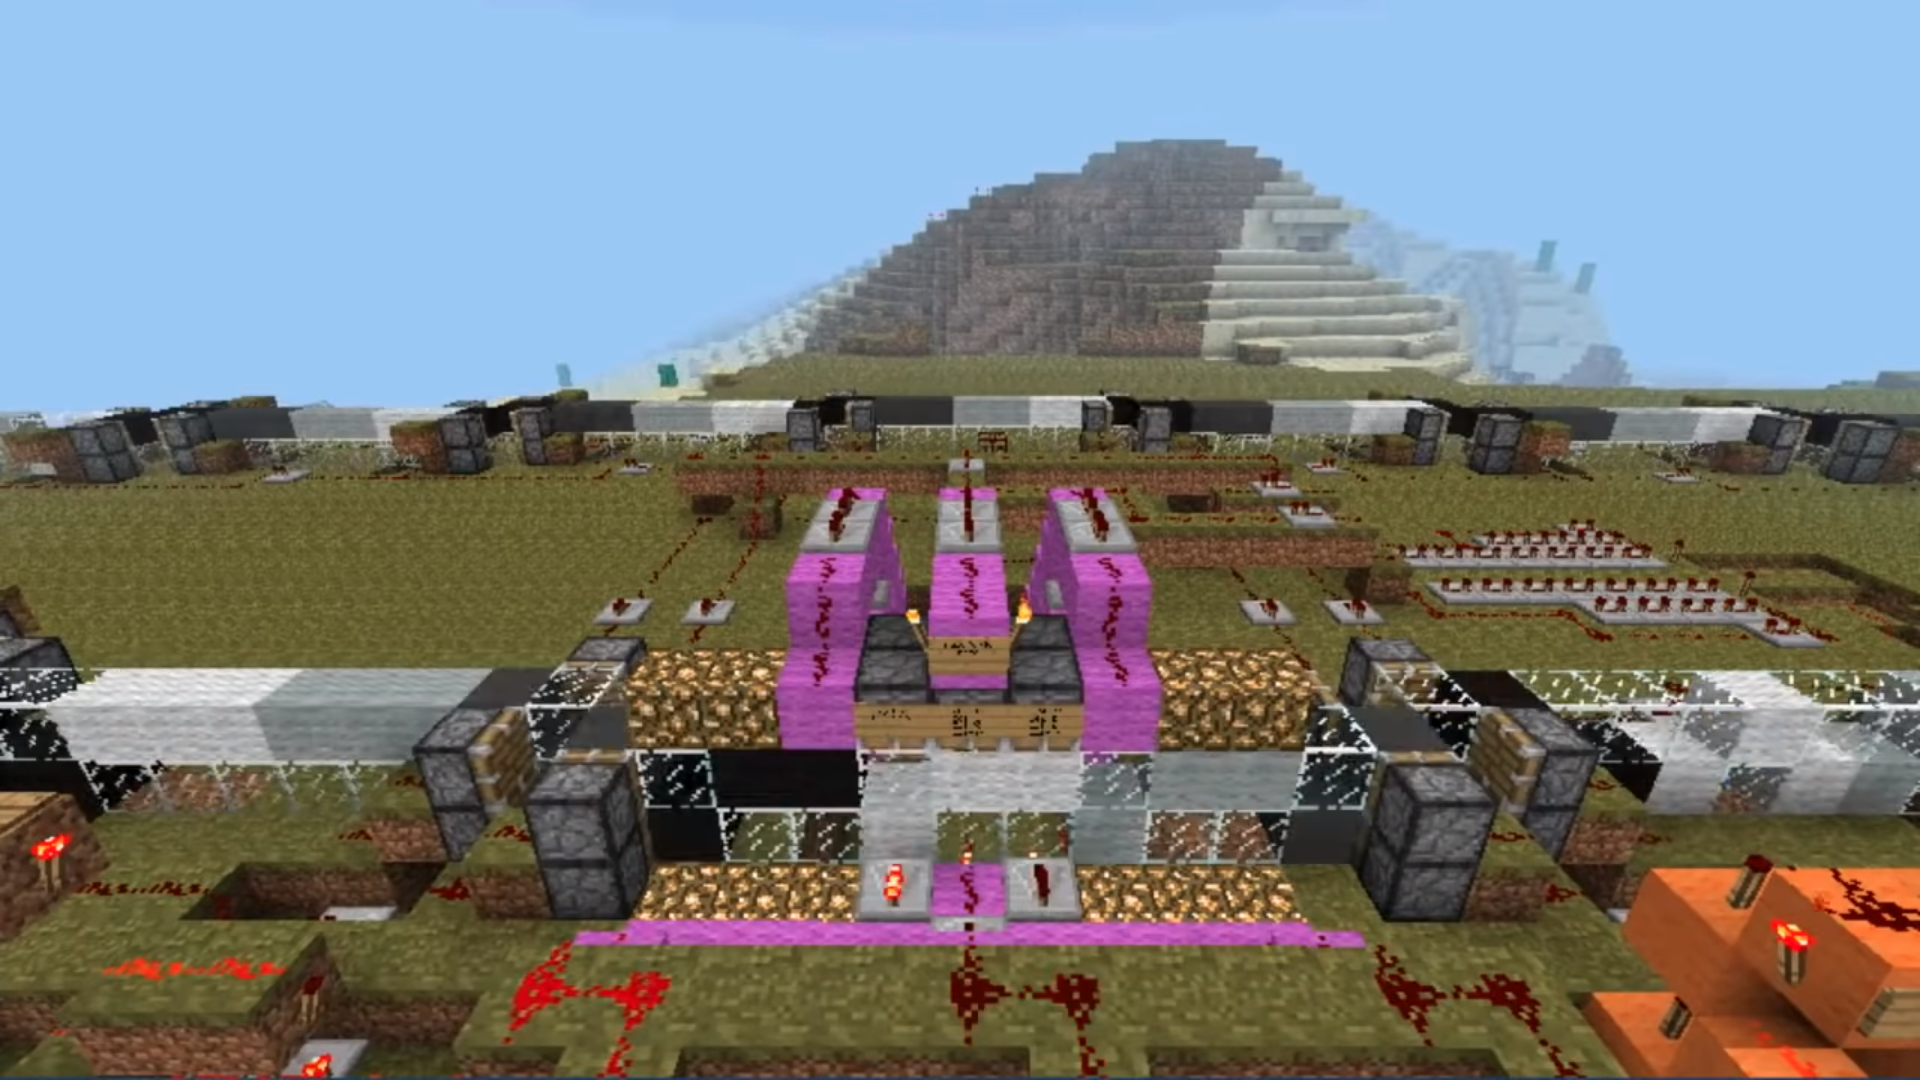
\includegraphics[height=2.2cm]{figures/turing_minecraft2.png}}
        \end{column}
    \end{columns}

    \begin{columns}
        \begin{column}{.6\hsize}
            {MS PowerPoint}
            {\footnotesize
            \begin{itemize}
                \myitem Tom Wildenhain, 2017 {\color{blue} \hyperlink{frame:przypisy}{(15)}}
                \myitem Wykorzystanie hiperłączy i animacji do zbudowania maszyny Turinga
            \end{itemize}
            }
        \end{column}
        \begin{column}{.45\hsize}
            {\hspace{0cm}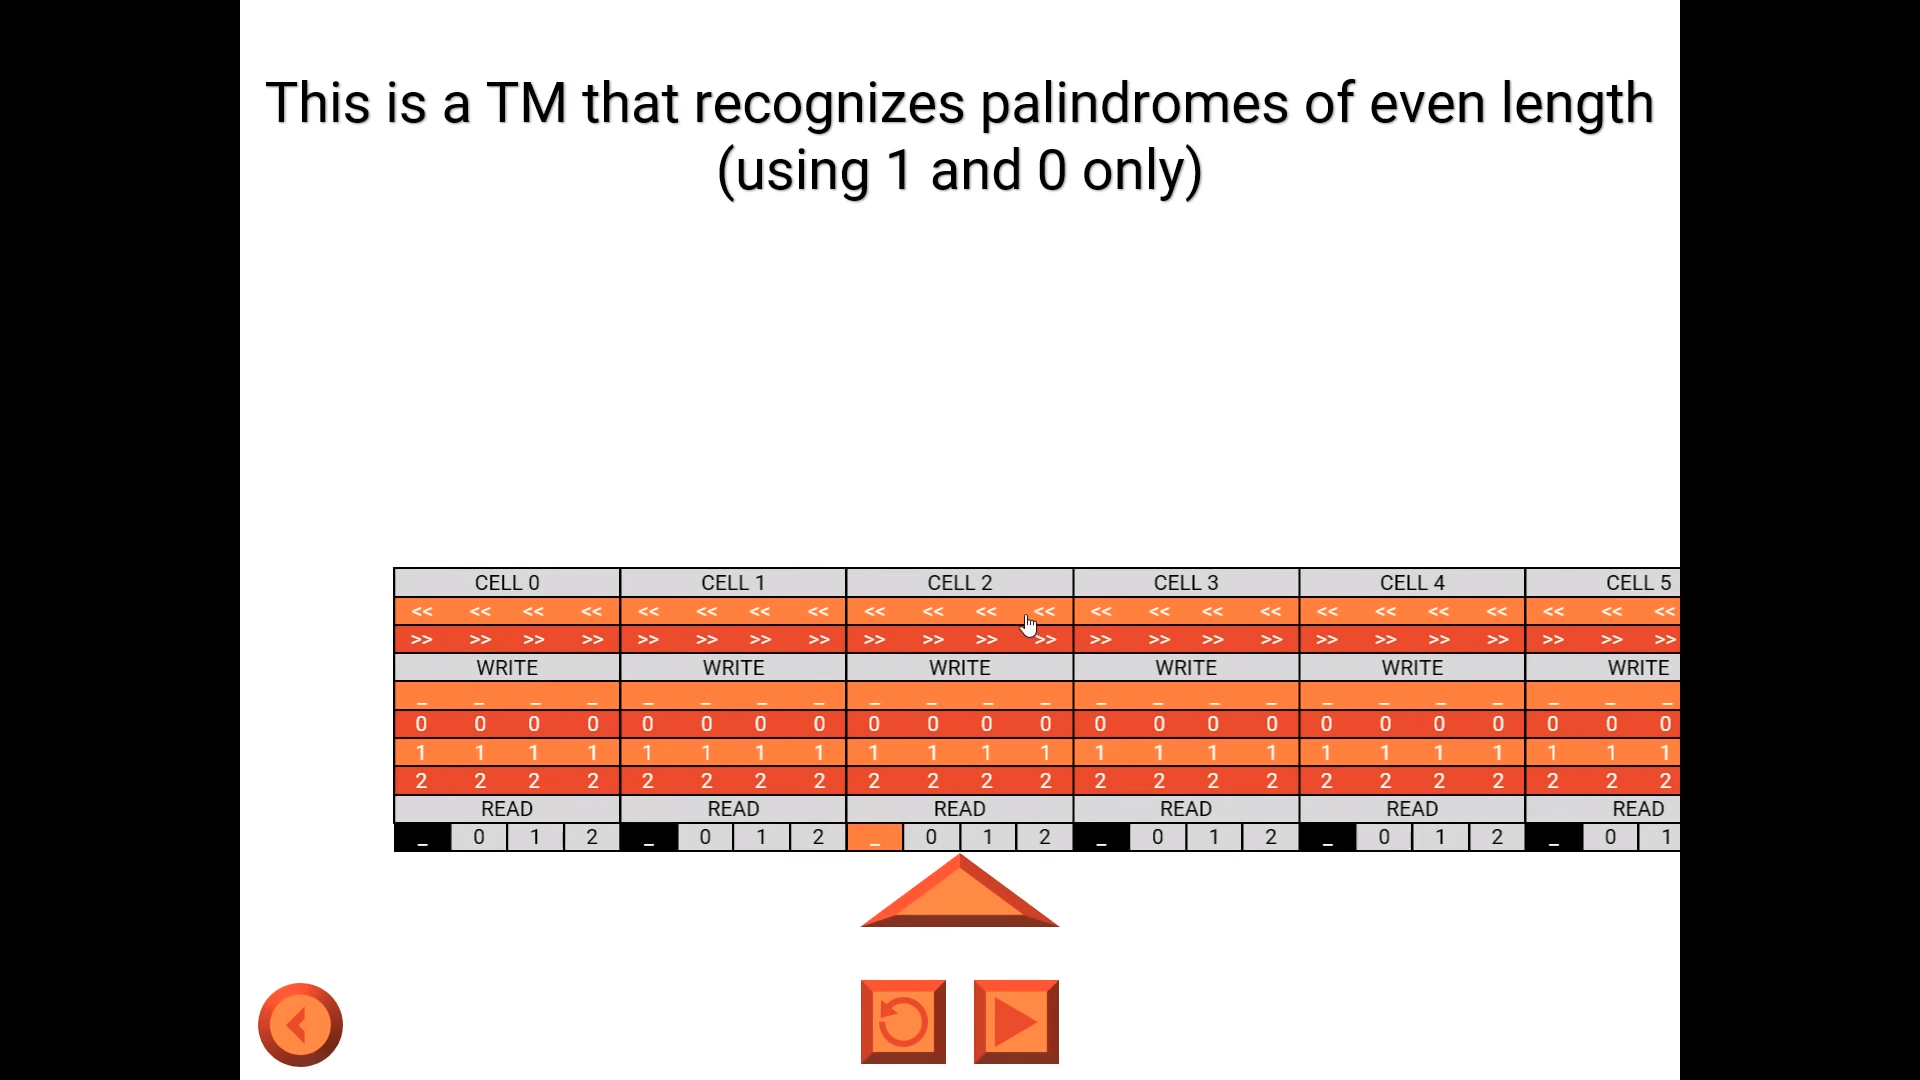
\includegraphics[height=2.2cm]{figures/turing_powerpoint.png}}
        \end{column}
    \end{columns}

    \begin{columns}
        \begin{column}{.6\hsize}
            {Magic the Gathering}
            {\footnotesize
            \begin{itemize}
                \myitem Alex Churchill, Stella Biderman, Austin Herrick, 2019 {\color{blue} \hyperlink{frame:przypisy}{(16)}}
                \myitem Statystyki niektórych kart przechowują informację o położeniu na taśmie maszyny Turinga (demonstracja autorstwa BecauseScience {\color{blue} \hyperlink{frame:przypisy}{(17)}})
            \end{itemize}
            }
        \end{column}
        \begin{column}{.45\hsize}
            {\hspace{0cm}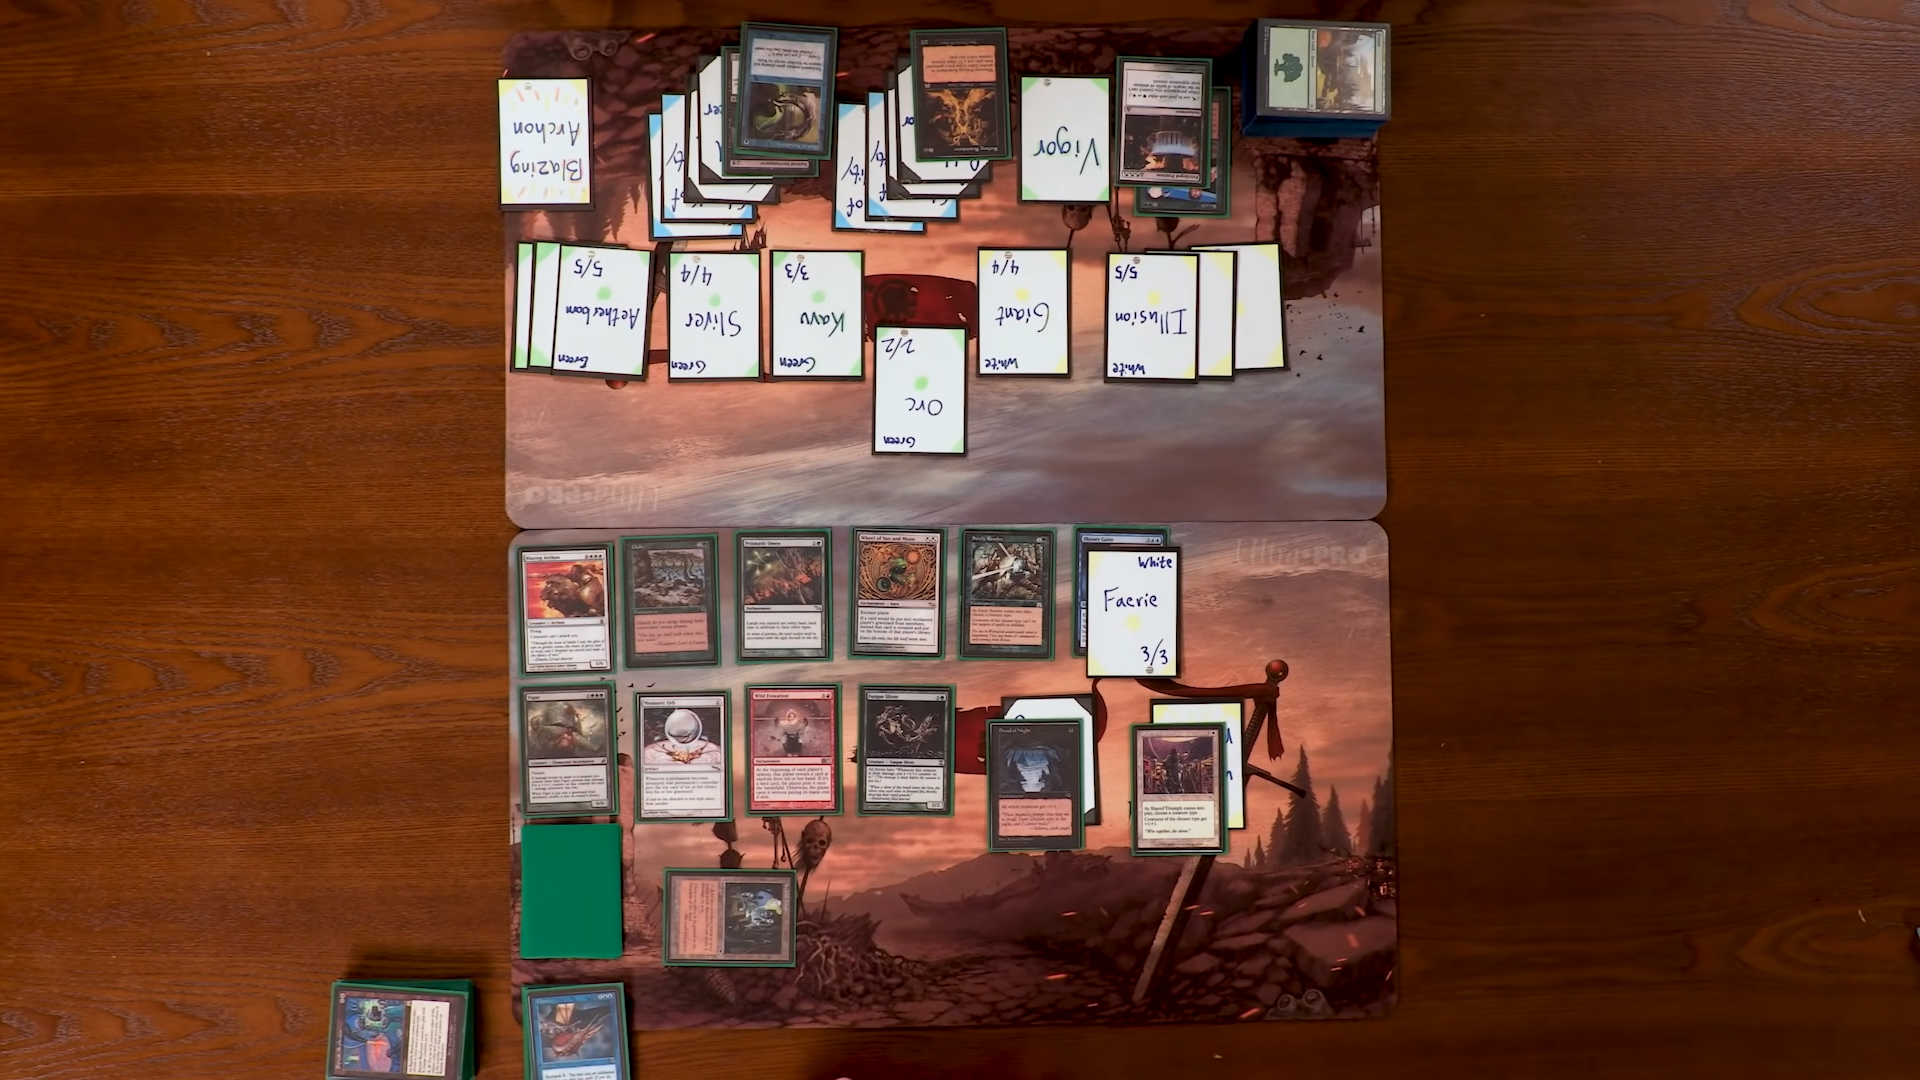
\includegraphics[height=2.2cm]{figures/turing_mtg.png}}
        \end{column}
    \end{columns}

\end{frame}

% \begin{frame}{\hypertarget{frame:przypisy}{Przypisy}}
	\vspace*{0.1cm}
	{\small
    (1) https://pl.frwiki.wiki/wiki/INTERCAL \\
    (2) https://www.youtube.com/watch?v=hdHjjBS4cs8 \\
    (3) https://sites.google.com/site/visualbf/ \\
    (4) https://en.wikipedia.org/wiki/Befunge \\
    (5) https://shakespearelang.com/1.0/ \\
    (6) http://www.mike-worth.com/2013/03/31/baking-a-hello-world-cake/ \\
    (7) https://en.wikipedia.org/wiki/Esoteric\_programming\_language\#Piet \\
    (8) https://esolangs.org/wiki/Folders \\
    (9) https://en.wikipedia.org/wiki/Whitespace\_(programming\_language) \\
    (10) https://codegolf.stackexchange.com/a/57761 \\
    (11) https://codegolf.stackexchange.com/a/58762 \\
    (12) https://codegolf.stackexchange.com/a/57693 \\
    (13) https://codegolf.stackexchange.com/a/57641 \\
    (14) https://youtu.be/1X21HQphy6I \\
    (15) https://www.youtube.com/watch?v=uNjxe8ShM-8 \\
    (16) https://arxiv.org/abs/1904.09828 \\
    (17) https://www.youtube.com/watch?v=pdmODVYPDLA
	% \begin{itemize}
	% 	\item https://esolangs.org/wiki/Main\_Page	% https://esolangs.org/wiki/Main_Page
	% 	\item https://en.wikipedia.org/wiki/Esoteric\_programming\_language	% https://en.wikipedia.org/wiki/Esoteric_programming_language
	% 	\item https://hillelwayne.com/talks/esolangs/	% https://hillelwayne.com/talks/esolangs/
	% 	\item https://codegolf.stackexchange.com/	% https://codegolf.stackexchange.com/
	% 	\item https://matt-rickard.com/accidentally-turing-complete	% \item https://matt-rickard.com/accidentally-turing-complete
	% \end{itemize}
	}
\end{frame}

% \begin{frame}{Bibliografia}
	\vspace*{0.1cm}
	{\small
	\begin{itemize}
		\item https://esolangs.org/wiki/Main\_Page	% https://esolangs.org/wiki/Main_Page
		\item https://en.wikipedia.org/wiki/Esoteric\_programming\_language	% https://en.wikipedia.org/wiki/Esoteric_programming_language
		\item https://hillelwayne.com/talks/esolangs/	% https://hillelwayne.com/talks/esolangs/
		\item https://codegolf.stackexchange.com/	% https://codegolf.stackexchange.com/
		\item https://matt-rickard.com/accidentally-turing-complete	% \item https://matt-rickard.com/accidentally-turing-complete
	\end{itemize}
	}
\end{frame}


\begin{frame}[plain]{Bibliografia}
	\begin{center}
		\begin{itemize}
			\myitem L. Pijanowski. \textit{Przewodnik gier}. Iskry, 1978.
			\myitem J. Schaeffer, N. Burch, Y. Björnsson, A. Kishimoto, M. Müller, R. Lake, P. Lu, S. Sutphen. \textit{Checkers is solved}. 2007.
			\myitem J. Mańdziuk, M. Kusiak, K. Walędzik. \textit{Evolutionary-based heuristic generators for checkers and give-away checkers}. 2007.
			\myitem S. Russel, P. Norvig. \textit{Artificial Intelligence: A Modern Approach}. Pearson Education, Inc., 2010.
		\end{itemize}
	\end{center}
\end{frame}

\begin{frame}[plain]{}
	\begin{center}
		\large{Dziękuję za uwagę.}
	\end{center}
\end{frame}

% \begin{frame}[plain]{}
% \end{frame}
\begin{frame}{Implementacja algorytmu genetycznego}
    \begin{enumerate}
        \item \textbf{Osobniki} \\
        Ciągi wag w postaci tablic liczb całkowitych.
        \item \textbf{Ewaluacja} \\
        Pojedynek każdy-z-każdym (białe/czarne i na odwrót)
        \item \textbf{Selekcja} \\
        Ruletka (lepiej grające osobniki mają większą szansę na przejście)
        \item \textbf{Krzyżowanie} \\
        Pary rodziców mają po dwójce dzieci 
        \item \textbf{Mutacje} \\
        Szansa na wylosowanie nowej wartości losowej wag w ciągu.
    \end{enumerate}
\end{frame}


\end{document} 